\chapter{Глоссарий}
Основным понятиям в статистике и стохастическом моделировании является \emph{распределения случайной величины} или, более общо, \emph{распределения случайного объекта} (далее, под случайной величиной понимается любой случайный объект, реализации которого не обязательно суть вещественные числа) \cite{knuth2014art}. Ниже изложены основные теоретические сведения касающиеся случайных величин, а также задач в которых они возникают, в соответствии с монографиями \cite{Feller2013} и \cite{shiryaev2007prob}. 

\subsubsection*{Случайные величины и способы их задания} 
Для случайной величины $\xi$, принимающей значения в некотором пространстве $\mathcal{X}$, её распределением называется (см{.}~\cite{shiryaev2007prob}) вероятностная мера $\P_\xi(\cdot)$ на $\mathcal{X}$, такая что $\P_\xi(A)$ есть вероятность того что реализация $\xi$ попадет в множество $A \subset \mathcal{X}$\footnote{Строго говоря, $\mathcal{X}$ должно быть снабжено некоторой $\sigma$-алгеброй $\mathcal{F}$, и $\P_\xi$ должна быть определена только для $A \in \mathcal{F}$. Иначе говоря, тройка $(\mathcal{X}, \mathcal{F}, \P_\xi)$ должна образовывать вероятностное пространство.}. Как правило (см{.} \cite{Feller2013}),  выделяют следующие виды случайных величин 
\begin{itemize}[noitemsep, topsep=0pt, parsep=3pt]
    \item Дискретные случайные величины. В этом случае $\mathcal{X}$ представляет собой некоторое дискретное (конечное или счетное) множество. Например число выпадений монеты орлом при нескольких бросках (биномиальное распределение);  уровень образования у случайно выбранного человека (категориальное распределение); случайная величина которая принимает одно значение (вырожденное распределение);
    \item Одномерные непрерывные случайные величины\footnote{Здесь и далее под непрерывными случайными величинами подразумеваются абсолютно-непрерывные случайные величины, т.е. распределение которых имеет плотность относительно меры Лебега}. В этом случае $\mathcal{X} = \R$ или $\mathcal{X} \subset \R$ ненулевой меры. Такие величины используются для описания случайных времен, расстояний и т{.}д{.} Согласно \cite{knuth2014art} наиболее важными представителями являются: равномерное распределение $\Uniform(a; b)$ , нормальное распределение $\Normal(\mu, \sigma^2)$ и экспоненциальное распределение $\Exp(\lambda)$;
    \item Многомерные непрерывные случайные величины. В этом случае $\mathcal{X} \subseteq \R^d$, ненулевой меры. Во много многомерные случайные величины являются аналогами одномерных непрерывных случайных величин, однако решение стандартных задач, таких как моделирование или вычисление числовых характеристик затруднено из-за проклятия размерности \cite{donoho2000high}.  
\end{itemize}
Отдельное направление статистики работает с данными о направлении (англ{.} directional data), в связи с этим часто можно также отдельно выделить следующую категорию случайных величин.
\begin{itemize}[noitemsep, topsep=0pt, parsep=3pt]
    \item Случайные геометрические  примитивы (англ{.} geometrical random primitives). Примерами таких случайных величин служат случайные углы или случайные матрицы симметрий. Согласно \cite{pennec1999probabilities}, геометрической случайной величиной называется случайная величина принимающая значения на замкнутой и ограниченной поверхности в евклидовом пространстве (более общо---компактном Римановом многообразии). 
\end{itemize}

С точки зрения ПО, работа с распределением, как с вероятностной мерой, является неудобной, так как компьютер не может работать с произвольными множествами. Однако, как правило, с распределением можно связать некоторую функцию, которая полностью определяет распределение. Так, чтобы идентифицировать распределение дискретной случайной величины, достаточно знать \emph{функцию вероятности}, определяемую равенством \eqref{eq:distribution:pmf}.
\begin{equation}
    \label{eq:distribution:pmf}
    \pmf_\xi(x) = \P_\xi(\set{x}), \text{ т{.}е{.} вероятность того что $\xi = x,\ x\in \mathcal{X}$} \tag{pmf}
\end{equation}
Если на пространстве возможных значений $\mathcal{X}$ задана некоторая мера $\mu$, плотностью распределения $\P_\xi$ относительно $\mu$ называется\footnote{Условия существования плотности описываются теоремой Радона-Никодима, см{.} например \cite{lanchier2017stochastic}} такая функция $\pdf_\xi(x) \colon \mathcal{X} \to \R$, что выполнено тождество \eqref{eq:distribution:pdf}:
\begin{equation}
        \label{eq:distribution:pdf}
        \P_\xi(A)=\int_{A}\pdf_\xi(x)\dif \mu  \tag{pdf}
\end{equation}
В случае если $\mu$ это считающая мера, плотность $\pdf_\xi$ определяется равенством \eqref{eq:distribution:pmf}, в случае если $\mu = \mleb$, говорят просто о плотности непрерывной случайной величины/случайного вектора. 

Несмотря на то что плотность распределения полностью его характеризует, для того чтобы вычислять вероятности $\P_\xi(A)$ необходимо производить интегрирование (или суммирование), поэтому для некоторых задач представление распределения в виде плотности является неудобным. В частности, если $\xi$ --- случайная величина (дискретная или непрерывная) принимающие значения из $\R^d$, довольно часто приходится смотреть на вероятность попадания в некоторую ячейку $\interval{\mathbf{a}}{\mathbf{b}}$. Под ячейкой подразумевается множество:
$$
    \interval{\mathbf{a}}{\mathbf{b}} = \set{\begin{pmatrix}c_1\\\vdots\\c_d\end{pmatrix} \in \R^d | a_1<  c_1 \leq b_1, \cdots,a_d < c_d \leq b_d} 
$$
Для доступа к таким вероятностям эффективнее работать с \emph{функцией распределения случайной величины}, определяемой равенством  \eqref{eq:distribution:cdf}. 
\begin{equation}
    \label{eq:distribution:cdf}
    \cdf_\xi(\mathbf{x}) = \P_\xi(\interval{\mathbf{-\infty}}{\mathbf{x}}) \tag{cdf}
\end{equation}
В этом случае $\P_\xi(\interval{a}{b})$ выражается через значения $\cdf_\xi(\cdot)$ с помощью формулы включения-исключения \cite{Feller2013}. 

С понятием функции распределения тесно связано понятие квантильной функции. Для случайной величины $\xi$ со значениями из $\R$, её квантильная функция определяется равенством \eqref{eq:distribution:ppf} (подробно о различных определениях см{.}~в обзоре  \cite{delafortelle2106}).
\begin{equation}
    \label{eq:distribution:ppf}
    \omega_{\xi}(p) = \inf_{u}\set{\cdf_\xi(u) \geq p} \tag{ppf}
\end{equation}
Такое определение гарантирует, что случайная величина $\ppf_{\xi}(U), U \sim \Uniform[0;1]$ имеет такое же распределение как и сама величина $\xi$. В случае когда $\cdf_\xi(\cdot)$ строго возрастает на всей области определения, квантильная функция является обратной функцией $\ppf_\xi(\cdot) = \cdf_\xi^{-1}(\cdot)$.  Отдельно следует отметить что существуют обобщения понятия квантильной функции на случай случайных величин со значениями из $\R^d$ \cite{hallin2024multivariate}, однако для их вычисления необходимо решать уравнения в частных производных \cite{figalli2018continuity}. 

Существуют и другие функциональные характеристики распределения, многие из которых приходят из анализа выживаемости \cite{kleinbaum1996survival}. \emph{Функцией выживаемости} называется функция определяемая равенством \eqref{eq:distribution:sdf}.
\begin{equation}
    \label{eq:distribution:sdf}
    \sdf_\xi(\mathbf{x}) = 1 - \cdf_\xi(\mathbf{x}) \tag{sdf}
\end{equation}
Для случайных величин со значениями из $\R$,  функцией интенсивности отказов и кумулятивной функцией интенсивности отказов называются функции определяемые равенствами \eqref{eq:distribution:hrdf} и \eqref{eq:distribution:chdf} соответственно. 
\begin{align}
    \label{eq:distribution:hrdf}
    &\hrdf_\xi(x) = -\frac{\sdf_\xi'(x)}{\sdf_\xi(x)}; \tag{hrdf} \\
    \label{eq:distribution:chdf}
    &\chdf_\xi(x)=-\ln(\sdf_\xi(x)); \tag{chdf}
\end{align} 
 
Однако, некоторые распределения, например $\alpha$-устойчивые распределения \cite{Feller2013}, не допускают явного задания с помощью плотности или функции распределения, однако допускают задания с помощью так называемых \emph{интегральных преобразований}. Такие распределения все чаще возникают в современных моделях стохастического анализа, (см{.} например \cite{barndorff2018ambit}). В случае случайной величины $\xi$ со значениями из $\R$, её
\begin{itemize}
    \item Характеристической функцией $\xi$ называется преобразование Фурье, определяемое равенством \eqref{eq:distribution:cf}. 
    \begin{equation}
        \label{eq:distribution:cf}
        \varphi_{\xi}(u) = \int_{\R} \exp(itu) \P_\xi(\dif t), \quad u \in \R \tag{cf}
    \end{equation}
    \item Момент-производящей функцией называется преобразование определяемое равенством \eqref{eq:distribution:mgf}.
    \begin{equation}
        \label{eq:distribution:mgf}
        \MGF_{\xi}(u) = \int_{\R} \exp(tu) \P_\xi(\dif t), \quad u \in \R \tag{mgf}
    \end{equation}
\end{itemize}
Характеристическая функция всегда существует и полностью определяет распределение случайной величины~\cite{shiryaev2007prob}. В свою очередь, момент-производящая функция существует не всегда, но в тех случаях когда существует, также однозначно характеризует распределение. В случае когда $\xi$ принимает только неотрицательные значения, определены также преобразование Лапласа и преобразование Меллина, задаваемые равенствами \eqref{eq:distribution:lt} и \eqref{eq:distribution:mt} соответственно. 
\begin{align}    
    \label{eq:distribution:lt}
    &\Laplace_{\xi}(u) = \int_{\R_+} \exp(-tu) \P_\xi(\dif t), \quad u \in \R_{+} \tag{lt}\\
    \label{eq:distribution:mt}
    &\Mellin_{\xi}(u) = \int_{\R_{+}} t^u \P_\xi(\dif t), \quad u\in \R_{+} \tag{mt}
\end{align}
Эти преобразования также однозначно характеризуют распределение $\xi$ \cite{Feller2013}, \cite{galambos2004products}. В случае если $\xi$ многомерная случайная величина, также определяется характеристическая функция (см{.} \cite{shiryaev2007prob}), преобразования \eqref{eq:distribution:mgf}, \eqref{eq:distribution:lt}, \eqref{eq:distribution:mt} в некоторых ситуациях допускают обобщение на многомерный случай, см{.} например \cite{antipova2007inversion}. 

На \picref{fig:continuous-distributions-models} схематично изображены основные способы задания непрерывных вероятностных распределений, и связь между ними. В связи с тем что в теории многомерных квантилей нет результатов напрямую выражающих квантильные функции через плотности или интегральные преобразования, переходы которые имеют место быть только в одномерном случае, изображены пунктирными стрелками.



\begin{figure}[h!]
        \centering
        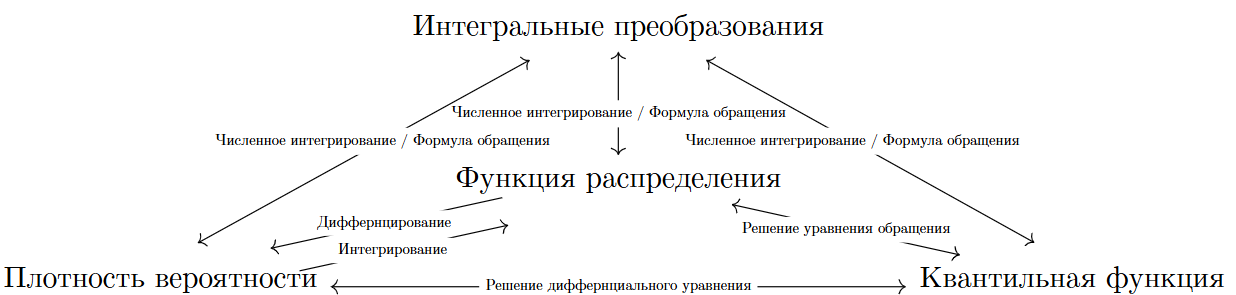
\includegraphics[width=\figurewidth]{distribution-characteristics}
        \caption{Способы задания непрерывных распределений}
        \label{fig:continuous-distributions-models}
    \end{figure}

\begin{remark*}
    Плотность и функция распределения непрерывной случайной величины со значениями в $\R^d$ связаны соотношениями
    \begin{equation}
      \pdf_{\xi}(\mathbf{x}) = \frac {\partial \cdf_\xi}{\partial x_1 \cdots \partial x_d}(\mathbf{x}) \quad 
      \cdf_{\xi}(\mathbf{x}) = \smashoperator[rl]{\int\limits_{\interval{\mathbf{-\infty}}{\mathbf{x}}}}\pdf_{\xi}(\mathbf{t})\dif \mathbf{t}  
    \end{equation}
    Формулы обращения для интегральных преобразований представлены в \cite{shiryaev2007prob}, \cite{galambos2004products}. Отдельно стоит отметить, что в работе \cite{steinbrecher2008quantile} показано как можно вычислять квантильную функцию по плотности распределения и наоборот, не прибегая к вычислению функции распределения. Этот подход может оказаться полезным при работе с достаточно сложными плотностями.
\end{remark*}


\subsubsection*{Семейства вероятностных распределений}
В задачах статистики, как правило, оперируют не с одним каким-то конкретным распределением, а с набором распределений, из которого надо выбрать наиболее подходящее, или проверить какую-то гипотезу. Более строго, \emph{параметрическим семейством распределений} называется некоторое множество $\set{\P_\theta}_{\theta \in \Theta}$ распределений, зависящих от скалярного или векторного параметра $\theta$, $\Theta$ --- множество возможных значений параметра \cite{Chernova2007ms}. 

Для любого распределения $\P_\xi$ случайной величины $\xi$ определено семейство локации и масштаба, т.е. семейство распределений всех аффинных преобразований величины $\xi$:
\begin{equation}
    \label{eq:family:loc-scale}
    \mathrm{loc}+ \mathrm{scale} \cdot\xi \sim\P_{(\mathrm{loc}, \mathrm{scale});}^{\xi}  \tag{loc-scale-family}
\end{equation}
где параметры $ \mathrm{loc}, \mathrm{scale}  \in \R$ для вещественнозначных случайных величин, и  $\mathrm{loc} \in \R^d,\, \mathrm{scale} \in \R^{d\times d}$ для векторозначных случайных величин. Примером такого семейства является семейство нормальных распределений~$\Normal(\mu, \sigma)$, определяемых равенством \eqref{eq:family:normal}.
\begin{equation}
    \label{eq:family:normal}
    \mu + \sigma \cdot \xi, \quad \xi \sim \mathcal{N}(0, 1), \text{ т.е. } \pdf_\xi(x) = \frac{1}{\sqrt{2\pi}}\exp\mleft(-\frac{x^2}{2}\mright) \tag{normal-family}
\end{equation}
Более общим понятием является понятие семейства замкнутого относительно действия группы, см{.} \cite{lehmann2006theory} и \cite{pace1997principles}. 

Другим, в некотором смысле ортогональным, понятием является понятие экспоненциального семейства распределений \cite{barndorff2014information}. Параметрическое семейство распределений $\set{\P_\theta}_{\theta \in \Theta}$ относится к экспоненциальному типу, если плотности (или функции вероятностей) которых можно записать в виде \eqref{eq:family:exponential}  \footnote{При этом требуется чтобы множество точек $\mathbf{x}$, в которых плотность отлична от 0, не зависело от параметра $\theta$}.
\begin{equation}
    \label{eq:family:exponential}
    f(\mathbf{x}|\theta) = \exp(\spr{\mathbf{T}(\mathbf{x})}{\vec{\eta}(\theta)}+ A(\mathbf{x}) + D(\theta) ) \tag{exp-family}
\end{equation}
Многие распространенные семейства распределений являются экспоненциальными, см{.} \cite{nielsen2009statistical} . Для моделей относящихся к экспоненциальным семействам существует богатая теория оценивания параметров \cite{lehmann2006theory}. Большой список параметрических семейств и связывающие их соотношения представлены в \cite{leemis2017univariate}.

Приведенные выше семейства интересны с точки зрения теоретической статистики. С точки зрения прикладной статистики, интерес представляют распределения, которые допускают гибкость в плане оценивания параметров: так, для нормального распределения два параметра не только локацию и масштаб, но и всю форму распределения, причем такое поведение присуще не только нормальному распределению.  Для того чтобы решить эту проблему, было предложено несколько  гибких семейств распределений, среди которых широко распространены семейство распределений Пирсона \cite{elderton1969systems} и металогическое семейство \cite{keelin2016metalog}. 


Отдельно стоит отметить, что многие параметрические семейства зачастую имеют несколько параметризаций, каждая из которых может быть удобна в том или ином контексте, например в работе \cite{prause1999generalized} приведены четыре параметризации для обобщенного гиперболического распределения. Множество других различных параметризаций для одних и тех же семейств собраны в базе проекта ProbOnto \cite{swat2016probonto}. 

 
\subsubsection*{Преобразования случайных величин}

Во многих моделях распределения могут быть составлены из более  простых распределений с помощью различных методов. В \cite{barndorff2014information} отмечается что, в контексте статистического вывода, любая модель для данных может рассматриваться как вероятностное распределение. Существует множество комбинировать и преобразовывать вероятностные распределения, интересная практическая реализация этого взгляда доступна в библиотеке Pomegranate, \cite{schreiber2018pomegranate}. Ниже рассмотрены основные способы для непрерывных вещественнозначных случайных величин, большинство которых относят к теории алгебры случайных величин, см{.} \cite{springer1979algebra}.
\begin{itemize}
    \item \emph{Аффинное преобразование}. Если случайная величина \(\xi\) имеет распределение с функцией плотности \(f_\xi(x)\), то плотность её линейного преобразования \(a\xi + b\) описывается равенством \eqref{eq:operations:affine};
    \begin{equation}
        \label{eq:operations:affine}
        f_{a+b\xi}(y) = \frac{1}{|a|} f_\xi\left(\frac{y - b}{a}\right), \quad a \neq 0. \tag{aff-tr}
    \end{equation}
    \item \emph{Биективное преобразование}. Плотность распределения случайной величины \(g(\xi)\), где \(g\) --- строго монотонная функция,определяется через обратную функцию \(g^{-1}(y)\) с помощью равенства \eqref{eq:operations:bijection}.
    \begin{equation}
        \label{eq:operations:bijection}
        f_{g(\xi)}(y) = f_\xi(g^{-1}(y)) \cdot \left|\frac{\dif}{\dif y} g^{-1}(y)\right|. \tag{bij-tr}
    \end{equation}
    Уравнение \eqref{eq:operations:affine} является частным случаем \eqref{eq:operations:bijection}. Для немонотонных функций распределение вычисляется с использованием разбиения на участки монотонности;
    \item \emph{Распределение суммы независимых случайных величин}  
    Если случайные величины \(\xi_1\) и \(\xi_2\) независимы\footnote{Т.е. $\P(\xi_1 \in B_1 \text{ и } \xi_2 \in B_2) = \P(\xi_1 \in B_1) \cdot \P(\xi_2 \in B_2)$ верно для всех $B_1, B_2 \subset \R$, являющихся борелевскими}, то плотность суммы \(\xi_1 + \xi_2\) вычисляется с помощью свёртки \eqref{eq:operations:sum}.
    \begin{equation}
        \label{eq:operations:sum}
        (f_{\xi_1} \oplus f_{\xi_2})(z) = \int_{\R} f_{\xi_1}(x) f_{\xi_2}(z - x) \, \dif x. \tag{sum-rv}
    \end{equation}
    \item \emph{Распределение произведения независимых случайных величин}. Для независимых случайных величин $\xi_1$ и $\xi_2$, плотность их произведения $\xi_1\cdot\xi_2$ задается с помощью мультипликативной свертки \eqref{eq:operations:prod}.
    \begin{equation}
        \label{eq:operations:prod}
        (f_{\xi_1} \odot f_{\xi_2})(z) = \int_{\R} \frac{1}{|x|} f_{\xi_1}(x) f_{\xi_2}\left(\frac{z}{x}\right) \, \dif x. \tag{prod-rv}
    \end{equation}
\end{itemize}

\noindent Другие две важные операции возникают при работе со случайными векторами --- маргинализация (взятие проекции) и вычисление порядковых статистик. Умение вычислять такие преобразования позволяет получать точные оценки качества в некоторых моделях статистического вывода. 
\begin{itemize}
    \item \emph{Проекции}. Для случайного вектора \(\xi=(\xi_1, \xi_2, \ldots, \xi_d)\)  (с возможно зависимыми компонентами) с  функцией распределения $\cdf_{\xi}(\mathbf{x})$, функция распределения случайного  подвектора $(\xi_{i_1}, \ldots,\xi_{i_k})$, описывается пределом \eqref{eq:operations:proj}
    \begin{equation}
        \label{eq:operations:proj}
        \cdf_{\Pr(\xi; i_1,\ldots,i_k)}(x_{i_1},\ldots, x_{i_k}) = \lim_{\substack{x_i \to+\infty\\ i \neq i_1,\ldots,i_k}}\cdf_{\xi}(x_1,\ldots,x_d)  \tag{proj-tr}
    \end{equation}
    \item \emph{Длины и углы}. Как правило, под случайными вектором понимается случайный элемент $\R^d$ представимый своими координатами. Однако, в некоторых ситуациях (см. например \cite{hernandez2017general}) куда удобнее оперировать со сферическими или другими координатами. В этом случае работает многомерный аналог формулы \eqref{eq:operations:bijection}.
\end{itemize}
Отдельно стоит отметить что важную роль играют порядковые статистики (см{.} \cite{lehmann1975statistical}). Если компоненты случайного вектора \(\xi=(\xi_1, \xi_2, \ldots, \xi_d)\) независимы и одинаково распределены с плотностью распределения $\pdf(x)$ и функцией распределения $\cdf(x)$, то их порядковые статистики \( \xi_{(1:d)} \leq \xi_{(2:d)} \leq \ldots \leq \xi_{(n)} \) имеют плотности, описываемые равенством \eqref{eq:operations:k-stat}.
\begin{equation}
    \label{eq:operations:k-stat}
    f_{\xi_{(k)}}(x) = \frac{n!}{(k-1)!(n-k)!} [F(x)]^{k-1} [1 - F(x)]^{n-k} f(x). \tag{ord-stat}
\end{equation}


Помимо трансформации одного распределения в другое и алгебраических операций над распределениями, еще одним способом образования   сложного распределения из нескольких простых является образование \emph{смесей}. Смеси используется для построения сложных вероятностных моделей, в которых присутствуют скрытые параметры и широко применяются в кластерном анализе и для изучения ядерных оценок плотности. Можно выделить два класса смесей; дискретные и непрерывные. 
\begin{itemize}
    \item \emph{Дискретная смесь}. Под дискретной смесью подразумевают комбинацию конечного числа распределений, каждое из которых взвешено определённым коэффициентом. Функция распределения дискретной смеси случайных величин $\xi_1, \ldots, \xi_n$ с весами $\vw = (w_1,\ldots, w_n)$ задаётся равенством \eqref{eq:operations:dmix};
    \begin{equation}
        \label{eq:operations:dmix}
        \cdf_{\mathrm{mix}(\vw; \xi)}(x) = \sum_{i=1}^n w_i \cdf_{\xi_i}(x), \quad \sum_{i=1}^n w_i = 1\tag{dmix}
    \end{equation}

    \item \emph{Непрерывная смесь} является непрерывным аналогом дискретной смеси. Пусть $F(x \,|\, \theta)$ семейство плотностей, зависящее от параметра $\theta \in \Theta \subset \R^n$. Если на $\Theta$ задано некоторое распределение параметров с плотностью $\omega(\theta)$, непрерывная смесь плотностей $F(x \, | \,\theta)$ определяется равенством \eqref{eq:operations:cmix}
    \begin{equation}
        \label{eq:operations:cmix}
        \cdf_{\mathrm{mix}(\omega; \cdf_\xi(\cdot |\theta))}(x) = \int_{\Theta} \cdf_{\xi}(x \mid \theta) \cdot w(\theta)\dif \theta, \tag{cmix}
    \end{equation}
    В данном случае параметр \(\theta\) рассматривается как случайная величина с заданным распределением.
\end{itemize}
Общая теория смесей в абстрактном случае и конкретные примеры приведены в работе \cite{Chandra1977absmix}. 

В приложениях часто возникают понятия цензурированных и урезанных распределений \cite{famoye1995continuous}. Для распределения $\P_{\xi}$ случайной величины $\xi$ принимающей вещественные значения, урезанным называется условное распределение, определяемое равенством \eqref{eq:family:truncated}. 
\begin{equation}
    \label{eq:family:truncated}
    \P_{\mathrm{Truncated}(\xi, L,R)}(B)=\frac{\P_{\xi}([L; R] \cap B)}{\P_{\xi}([L; R])} \tag{truncated-dist}
\end{equation}
Распределение \eqref{eq:family:truncated} это условное распределение $\xi$ если априори известно, что значение $\xi$ лежит в отрезке $[L; R]$. В свою очередь, цензурированным на отрезке $[L; R]$ распределением называется распределение случайной величины, определяемой равенством \eqref{eq:family:censored}. 
\begin{equation}
    \label{eq:family:censored}. 
    \mathrm{Censored}(\xi, L,R)=\begin{cases}
        L  & \xi < L \\
        \xi & L \leq \xi \leq R \\
        R & R < \xi 
    \end{cases} \tag{censored-dist}
\end{equation}
Такие распределения часто возникают в задачах регрессионного анализа, см{.} \cite{breen1996regression}.

\subsubsection*{Числовые характеристики вероятностных распределений}
Для анализа моделей важную роль играют не только функциональные, но и числовые характеристики распределений. Согласно \cite{famoye1995continuous}, \cite{weisberg1992central}, для случайной величины $\xi$ со значениями из $\R$ можно выделить следующие характеристики. 
\begin{itemize}
    \item Меры центральной тенденции, описывающие, вокруг какого значения сконцентрированы реализации случайной величины.
    \begin{itemize}[noitemsep, parsep=0pt,topsep=0pt]
        \item \emph{Математическое ожидание}. Для случайной величины $\xi$, её математическое ожидание определяется равенством~\eqref{eq:numchar:mean};
        \begin{equation}
            \label{eq:numchar:mean}
            \E[\xi] = \int_{\R}x \P_\xi(\dif x) \tag{mean}            
        \end{equation}
        \item \emph{Медиана}. Для случайной величины $\xi$, её медиана определяется как множество всех значений $m$, таких что $F_\xi(m)=\frac{1}{2}$, иначе говоря, медиана определяется равенством \eqref{eq:numchar:med}.
        \begin{equation}
            \label{eq:numchar:med}
            \Med[\xi] = \cdf_{\xi}^{-1}\mleft(\tfrac{1}{2}\mright) \tag{med}
        \end{equation}
        В некоторых случаях, в качестве медианы берут какое-то конкретное значение из множества $ \cdf_{\xi}^{-1}(\tfrac{1}{2})$, такое значение называется \emph{точной медианой} \cite{weisberg1992central}; 
        \item \emph{Мода}. Для случайной величины $\xi$ её мода определяется равенством \eqref{eq:numchar:mode}
        \begin{equation}
            \label{eq:numchar:mode}
            \Mode[\xi] = \argmax_{\R} f_\xi(x) \tag{mode}
        \end{equation}
        где $f_\xi(x)$ это функция вероятности, если $\xi$ --- дискретная случайная величина, и плотность, если $\xi$ непрерывная случайная величина.
    \end{itemize}
    \item Меры разброса (иногда меры рассеивания) указывают на склонность величины отклоняться от своего  центрального значения.
        \begin{itemize}[noitemsep, parsep=0pt,topsep=0pt]
            \item \emph{Дисперсия} и \emph{среднеквадратичное отклонение} определяются равенствами \eqref{eq:numchar:std} и \eqref{eq:numchar:std} соответственно;
            \begin{align}    
                \label{eq:numchar:var}
                &\D[\xi] = \E[(\xi - \E[\xi])^2]; \tag{var}\\
                \label{eq:numchar:std}
                &\std[\xi] = \sqrt{\D[\xi]} \tag{std}
            \end{align}
            \item \emph{Среднее абсолютное отклонение} определяются равенством \eqref{eq:numchar:mad}.
            \begin{equation}
                \label{eq:numchar:mad}
                \mad[\xi] = \E[\abs{\xi - \E[\xi]}] \tag{mad}
            \end{equation}
            \item \emph{Межквартильный размах} определяется равенством \eqref{eq:numchar:iqr}.
            \begin{equation}
                \label{eq:numchar:iqr}
                \IQR[\xi] = \ppf_{\xi}(0.75) - \ppf_\xi(0.25) \tag{iqr}
            \end{equation}
        \end{itemize} 
    \item Меры скоса---мера асимметрии распределения относительно среднего значения.
    \begin{itemize}[noitemsep, parsep=0pt,topsep=0pt]
        \item Коэффициент скоса определяется равенством \eqref{eq:numchar:skew};
        \begin{equation}
            \label{eq:numchar:skew} 
            \Skew[\xi] = \frac{\E[(\xi - \E[\xi])^3]}{\std^3[\xi]} \tag{skew}
        \end{equation}
        \item Коэффициент скоса Пирсона определяется равенством \eqref{eq:numchar:skew-pearon};
        \begin{equation}
            \label{eq:numchar:skew-pearon} 
            \mathrm{Skew}^{\mathrm{P}}[\xi] = \frac{\E[\xi] - \Med[\xi]}{\mad[\xi]} \tag{pskew}
        \end{equation}
        \item Обобщенный коэффициент скоса Грюневельда определяется равенством \eqref{eq:numchar:skew-pearon}.
        \begin{equation}
            \label{eq:numchar:skew-grunn} 
            \gamma(u) =\frac{\ppf_\xi(1 - u) + \ppf_\xi(u) - 2 \ppf_\xi\mleft(\frac{1}{2}\mright)}{\ppf_\xi(u) - \ppf_\xi(1 - u)} \quad \tfrac{1}{2} <u<1 \tag{qskew}
        \end{equation}
    \end{itemize}
    \item Меры эксцесса и тяжести хвостов
    \begin{itemize}[noitemsep, parsep=0pt,topsep=0pt]
        \item \emph{Коэффициент эксцесса} измеряет степень  остроты вершины распределения и определяется равенством \eqref{eq:numchar:kurt}.
        \begin{equation}
            \label{eq:numchar:kurt}
            \Kurt[\xi] = \frac{\E[(\xi - \E[\xi])^4]}{\std^4[\xi]} - 3 \tag{kurt}
        \end{equation}
    
        \item \emph{Квантильный коэффициент эксцесса} является квантильным аналогом стандартного коэффициента эксцесса \cite{ruppert1987kurtosis} и определяется равенством \eqref{eq:numchar:kurt-q};
        \begin{equation}
            \label{eq:numchar:kurt-q} 
            \kappa(u, v) = \frac{\ppf_\xi(1-u) - \ppf_\xi(u)}{\ppf_\xi(v) - \ppf_\xi(v)}, \quad 0<u<v<\frac{1}{2} \tag{qkurt}
        \end{equation}
    
        \item \emph{Экспонента хвоста} определяется для распределений, функция выживания которых убывает согласно степенному закону, как число $\alpha$ при котором верна асимптотическая эквивалентность \eqref{eq:numchar:tail-idx}.
        \begin{equation}
            \label{eq:numchar:tail-idx} 
            \sdf_{\xi}(x) \sim x^{-\alpha}, \quad x \to\infty. \tag{tail-idx}
        \end{equation}
        В общей ситуации отдельно определяется индекс для левого хвоста и для правого хвоста.
    \end{itemize}
\end{itemize}

Также, для случайной величины $\xi$ и натурального числа $n \in \N$ определены моменты, центральные моменты ($m_n$ и $\mu_n$ соответственно в равенстве \eqref{eq:numchar:moments}), абсолютные моменты, абсолютные центральные моменты ($v_n$ и $\nu_n$ в равенстве \eqref{eq:numchar:a-moments}) и факториальные моменты ($\kappa_n$ в равенстве \eqref{eq:numchar:f-moments}) порядка~$n$. На основе этих характеристик можно производить оценку параметров распределения.
\begin{align}
    \label{eq:numchar:moments}
    &m_n = \E[\xi^n] &&\mu_n = \E[\mleft(\xi - \E[\xi]\mright)^n] \tag{moment}\\
    \label{eq:numchar:a-moments}
    &v_n =\E[\abs{\xi}^k],&& \nu_n=\E[\abs*{\xi - \E[\xi]}^n]\tag{abs-moment}\\
    \label{eq:numchar:f-moments}
    &\kappa_n = \E[\xi(\xi-1)(\xi-2)\ldots(\xi-n+1)] \tag{fact-moment}
\end{align}
Обобщением моментов являются так называемые $L$-моменты \cite{hosking2014moments} и их квантильные аналоги $LQ$-моменты \cite{mudholkar1998lq}.  

Другое семейство числовых характеристик приходит из области теории информации, см{.} например монографию \cite{kullback1997information}. Далее, подразумевается что $\xi$ необязательно вещественнозначная случайная величина, со значениями из некоторого пространства $\mathcal{X}$ и под плотностью подразумевается плотность в смысле \eqref{eq:distribution:pdf}.
\begin{itemize}
    \item \emph{Энтропия} распределения с плотностью $p$ относительно меры $\mu$ определяется равенством \eqref{eq:numchar:entropy}
    \begin{equation}
    \label{eq:numchar:entropy}
        H_r(p) = -\int_\mathcal{X}p(x)\log_rp(x) \dif \mu \tag{entr}
    \end{equation}
    \item \emph{Кросс-энтропия} из распределения с плотностью $p$ в распределение с плотностью $q$ определяется равенством \eqref{eq:numchar:entropy}
    \begin{equation}
        \label{eq:numchar:croos-entr}
        CE_r(p \| q) = -\int_\mathcal{X}q(x)\log_rp(x) \dif \mu \tag{cross-enrt}
    \end{equation}
    \item \emph{KL-дивергенция} является мерой расхождения между двумя распределениями с плотностями $p$ и $q$ и определятся равенством \eqref{eq:numchar:kl-div}
    \begin{equation}
        \label{eq:numchar:kl-div}
        \mathcal{D}(p \| q) = - \int_\mathcal{X}q(x)\log_r\frac{p(x)}{q(x)}\dif\mu \tag{kl-div}
    \end{equation}
\end{itemize}
Методы из теории информации активно применяются в статистике, см{.} например \cite{amari2016information}. В частности, зачастую рассматривают обобщенный вариант KL-дивергенции ---  \emph{\(f\)-дивергенцию}, которая определяется для любой выпуклой функции $f \colon \R_{+} \to \R$ равенством \eqref{eq:numchar:f-div}.
\begin{equation}
    \label{eq:numchar:f-div}
    \mathcal{D}_f(p \| q) = \int_{\R} q(x) f\mleft(\frac{p(x)}{q(x)}\mright) \dif x \quad \tag{f-div}
\end{equation}
С информационными характеристиками тесно связана информация Фишера. Для параметрического семейства плотностей $f(x; \theta), \theta \in \Theta \subseteq \R$, информация Фишера это функция от параметра, задаваемая равенством \eqref{eq:numchar:fisher-inf}. 
\begin{equation}
    \label{eq:numchar:fisher-inf}
    \mathcal{I}(\theta) = \E\left[\left(\frac{\partial}{\partial \theta} \log \pdf_\xi(x; \theta)\right)^2\right] \tag{FI}
\end{equation}
   

\subsubsection*{Способы моделирования вероятностных распределений} 

Для вычисления метрик качества и моделирования поведения вероятностных систем необходимо уметь производить стохастическое моделирование случайных величин. Согласно \cite{hormann2013automatic}, для генерации выборок можно выделить три основных метода:
\begin{itemize}[noitemsep, parsep=0pt, topsep=0pt]
    \item \emph{Метод обратного преобразования}, который базируется на том факте, что для случайной величины $\xi$ с квантильной функцией $\ppf_{\xi}(p)$, распределение случайной величины $\ppf_{\xi}(U), U \sim \Uniform(0;1)$ будет совпадать с распределением $\xi$. 

    \item \emph{Метод декомпозиции}, который используется для генерации выборок из смешанных распределений. Общая идея заключается в том, что сначала генерируется значение параметра (например номер кластера), а затем уже случайная величина при условии зафиксированного значения параметра. 
    
    \item \emph{Метод отбора (rejection sampling)}, который используют когда предыдущие два метода не могут быть использованы. Этот метод значительно медленнее предыдущих и при его использовании возникает много нюансов, но для его использования необходим доступ только к плотности распределения. 
\end{itemize}
При этом дискретные распределения требуют отдельного рассмотрения. Существуют также методы основанные на методе отбора, для генерации выборок из распределений заданных с помощью интегральных преобразований.  При этом, нередки ситуации, плотность распределения \(\pdf_\xi(x)\) известна только с точностью до нормализующей константы или если требуется производить генерацию в сложных или многомерных пространствах. Для таких случаев разработаны методы на основе марковских цепей Монте-Карло (MCMC). Суть метода заключается в том, что на пространстве реализаций надо завести некоторое случайное блуждание, которое в пределе будет давать желанное распределение, детали см{.} например в книге \cite{liang2011advanced}. 

\subsubsection*{Примеры вероятностных моделей в PySATL}

В заключение этого раздела отметим, что поддержка работы с представленными ранее объектами является необходимой для PySATL в рамках существующих и будущих проектов. Пакет \texttt{MPEst}\footnote{\url{https://github.com/PySATL/MPEst}} использует различные числовые характеристики, такие как L-моменты для оценок параметров в моделях смеси.\\ Пакет \texttt{NMVMEstimation}\footnote{\url{https://github.com/PySATL/PySATL_NMVM_Module}} занимается специальными видами непрерывных смесей и использует различные интегральные преобразования. Библиотека \texttt{Experiment}\footnote{\url{https://github.com/PySATL/pysatl-experiment}} использует базовые характеристики распределений для оценок мощностей статистических тестов методом Монте-Карло. С помощью арифметики распределений можно будет получать точные распределения статистик используемых при проверке гипотез  В ближайшем будущем планируется начать разработку библиотек для регрессионного анализа и оценки параметров, где также широко потребуется использование различных свойств и характеристик распределений.
